%%%%%%%%%%%%%
%  Ch1 : Generalities  %
%%%%%%%%%%%%%

\chapter{Introduction}
%\section{History}
%	Where does the piston comes from? Who invented this mechanism? Here is a short story:
%	
%	\begin{itemize}
%		\item[•] \textbf{1206 - Al Jazari:} first use of a crankshaft connected to a rod and a reciprocating piston to describe the principle of a suction pump. 
%		
%		\item[•] \textbf{1509 - Leonardo da Vinci:} first description of the principle of an engine without compression using a piston and a cylinder.
		
%		\item[•] \textbf{1665 - Father Ferdinand Verbiest:} Flemisch, he developed the first steam-powered vehicle.
	
%		\item[•] \textbf{1673 - Christian Huyghens:} designs the first idea of an internal combustion engine by using gunpowder to drive a pump.
		
%		\item[•] \textbf{1690 - Denis Papin:} developed the first piston steam engine.
		
%		\item[•] \textbf{1690 - Denis Papin:} developed the first piston steam engine.
%	\end{itemize}

\section{Classification}
	We find a large amount of engines in the market, small, large, different types, ... But some are dedicated to specific applications. First of all, an engine is an \textbf{energy converter} and has to satisfy some requirements (cheap, long lifetime, quick start, ...). According to the type of engines, some of them are better fulfilled. Piston engines are on average rather good for all them. \\
	
	\begin{wrapfigure}[10]{l}{6cm}
	\vspace{-5mm}
	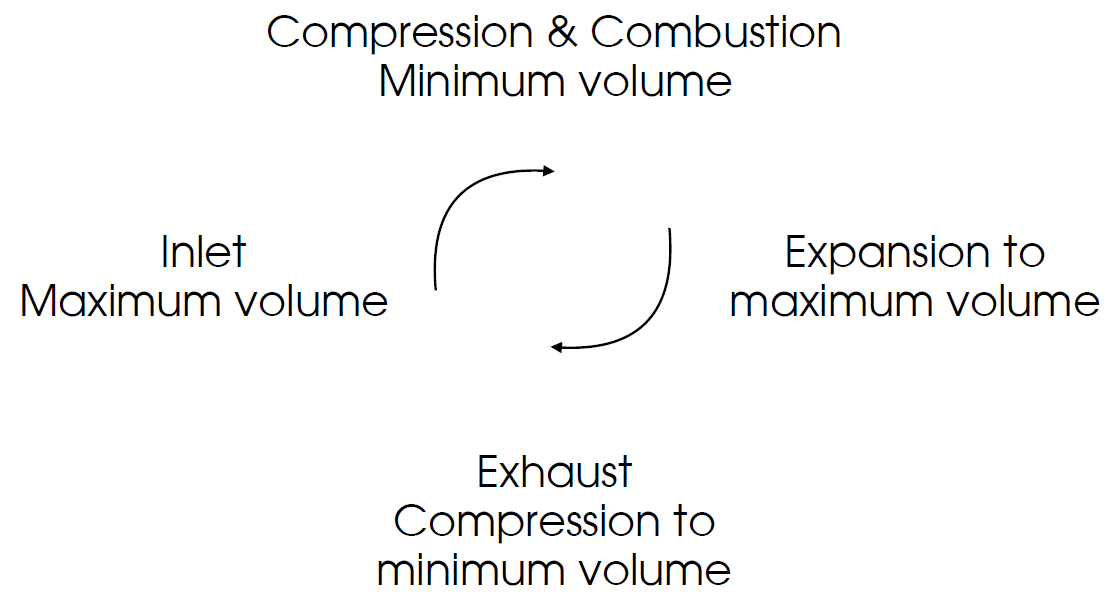
\includegraphics[scale=0.2]{ch1/1}
	\captionof{figure}{}
	\label{fig:1.1}
	\end{wrapfigure}
	The basic principle of an engine is based on the periodic production of mechanical work, using the reaction of fuel with the oxygen of air in a confined space, which produces heat and the pressure in a variable volume produces work:
	
	\begin{equation}
	\begin{aligned}
	&\mbox{chemical} \rightarrow m_f. \mbox{LHV} = Q_{in} \rightarrow thermal\\
	 &\rightarrow pV = nRT \rightarrow mechanical
	\end{aligned}	
	\end{equation}
	
	where LHV is the energy content of fuel, the Lower Heating Value. The \autoref{fig:1.1} represents the closed cycle for a 4 stroke engine but can be adapted for 2 stroke. \\
	
	Many classifications can be done following the size, the number of cylinder, ... But the mainly used one consists in 4 criteria:\\
	
	\begin{itemize}
		\item[•] \textbf{Heat source:} internal  or external (heat exchanger and working fluid in closed cycle)
		\item[•] \textbf{Mechanism:} piston-connecting rod-crankshaft, piston-piston rod-crosshead-connecting rod-crankshaft or rotary piston-excenter shaft
		\item[•] \textbf{Ignition:} spark ignition or compression ignition
		\item[•] \textbf{Strokes:} 4 strokes or 2
	\end{itemize}	 
	
	\subsection{Heat source}
		In this course, we only deal with the internal one. In this kind of source, fuel, air and the resulting combustion products are the working fluid. In the external type, the working fluid is in a closed cycle and transfers heat to an exchanger. The advantage of the external one is that we can use almost any fuel, have a more controlled combustion, but it is a more complex system and has less response to load change and there are more losses than the internal.   
		
	\subsection{Mechanism}
		
		\begin{center}
		\begin{minipage}{0.34\textwidth}
		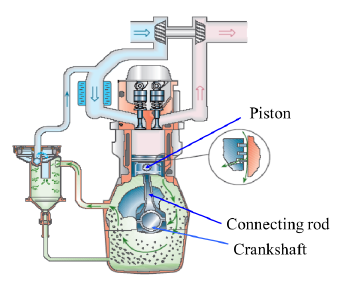
\includegraphics[scale=0.55]{ch1/2}
		\captionof{figure}{}
		\label{fig:1.2}
		\end{minipage}
		\begin{minipage}{0.28\textwidth}
		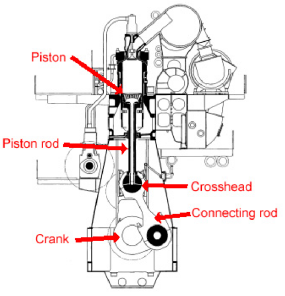
\includegraphics[scale=0.53]{ch1/3}
		\captionof{figure}{}
		\label{fig:1.3}
		\end{minipage}
		\begin{minipage}{0.35\textwidth}
		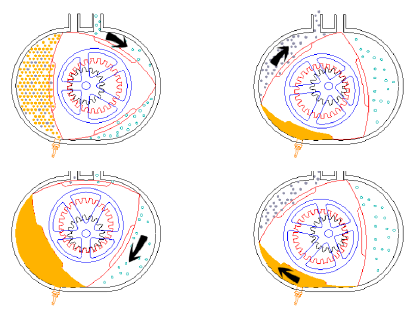
\includegraphics[scale=0.5]{ch1/4}
		\captionof{figure}{}
		\label{fig:1.4}
		\end{minipage}
		\end{center}
		
		\begin{itemize}
		\item[•]\autoref{fig:1.2} - The mostly used mechanism is composed of a \textbf{piston} connected to a \textbf{crankshaft} via a \textbf{connecting rod}. The crankshaft converts the reciprocating movement into a rotating one.\\
		\item[•]\autoref{fig:1.3} - Another mechanism where we have an additional \textbf{piston rod} between the piston and the connecting rod, coupled with a \textbf{crosshead}. This avoids the side forces on the piston due to the connecting rod movement. It is commonly used in large engines where side forces would produce too much wear (marine engines for example). \\
		\item[•]\autoref{fig:1.4} - The third famous mechanism is known as rotary or Wankel engine. It is based on an eccentric rotary motion. The triangular rotor forms 3 combustion chambers that undergo the 4 strokes of a classical engine. So, for one rotation we have 3 power strokes. It is compact and can be operated at higher speed giving a very high power to weight ratio, is smooth and balanced. The challenges relie in
the sealing of the combustion chamber, the higher heat transfer, the efficiency, and the emissions.
		\end{itemize}
		
	\subsection{Ignition}
		\begin{wrapfigure}[8]{l}{6cm}
		\vspace{-5mm}
		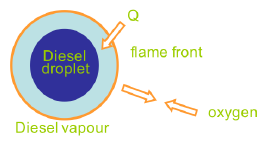
\includegraphics[scale=0.8]{ch1/5}
		\captionof{figure}{}
		\label{fig:1.5}
		\end{wrapfigure}
		The principle of \textbf{compression ignition engines} is to auto-ignite the fuel injected into a hot environment by compressing the air. Since the fuel is introduced close to ignition, the combustion is controlled by the mass diffusion of the fuel into the air. So, the work produced is controlled by the mass of injected fuel, air keeping a more or less constant rate. These engines work in lean conditions. \\
		
		\begin{wrapfigure}[7]{r}{6cm}
		\vspace{-15mm}
		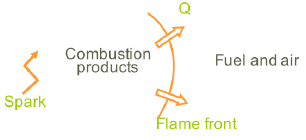
\includegraphics[scale=0.74]{ch1/6}
		\captionof{figure}{}
		\label{fig:1.6}
		\end{wrapfigure}
		The two major differences of \textbf{spark ignition} with compression ignition are the preparation of the mixture before or during the inlet and the ignition by mean of a spark. The combustion is characterised by a turbulent flame propagation. The work is controlled by the amount of air/fuel mixture and these operate in stoichiometric conditions. 
		
		\newpage
	\subsection{Strokes}
		\begin{wrapfigure}[12]{l}{8cm}
		\vspace{-5mm}
		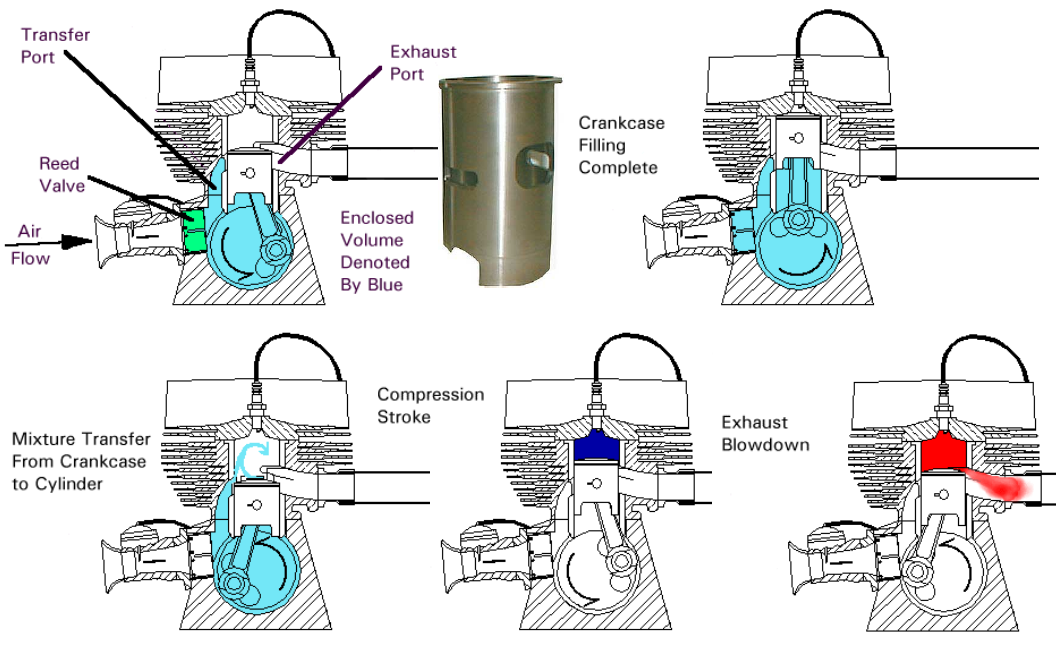
\includegraphics[scale=0.27]{ch1/7}
		\captionof{figure}{}
		\label{fig:1.7}
		\end{wrapfigure}
		In a \textbf{two stroke} cycle, there is one work producing stroke every rotation. In the case of spark ignition engine, the scavenging is done through a \textbf{transfer port}. The air/fuel mixture is slightly compressed to push the exhaust gas. Once the ports are sealed by the piston, begins the compression followed by combustion and expansion. The exhaust port is first open when expansion. For compression ignition, there is no loss of fuel since the scavenging is done pushing air via a compressor.\\
		
		\begin{wrapfigure}[12]{r}{6cm}
		\vspace{-5mm}
		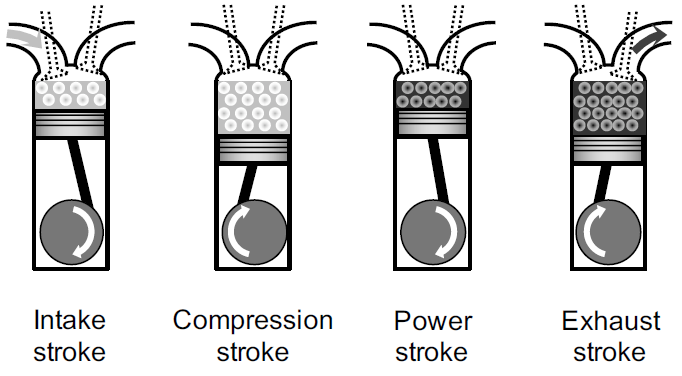
\includegraphics[scale=0.33]{ch1/8}
		\captionof{figure}{}
		\label{fig:1.8}
		\end{wrapfigure}
		The advantages of 2 stroke cycle is that it is more simple, produce more power-to-weight (1 power every rotation) with a more constant torque than the 4 stroke. But we have fuel losses (SI), we need to manage more heat and we must mix oil and fuel for lubrification. \\
		
		The \textbf{four stroke} cycle is composed of an intake, a compression, a combustion and an exhaust stroke. This induces one power stroke per two rotations.  